	\chapter{System (or Project) Design and Architecture}
        \section{System Block Diagram}
        The block Diagram of the proposed system is shown in the figure below: 
        \begin{figure}[h]
                \centering
                \includegraphics[width=1\textwidth]{img/chapter_6/Floor_plan_generation_block_diagram.png}
                \caption{Block Diagram of Floor Plan Generation}
                \label{fig: Block Diagram of Floor Plan Generation}
        \end{figure}
        \pagebreak 
        \section{Generation}
                From a given parcel land structure to a well furnished floor plan and its 3D view, we go through following main steps:
                \begin{enumerate}[label=\alph*.]
                        \item Footprint generation from parcel land structures.
                        \item Room split generation from selected Footprint.
                        \item Well furnished floor plan from selected room split.
                        \item 3D view of finally selected well furnished floor plan.
                \end{enumerate}
                \subsection{Foot-print generation}
                        This is the first step in generation pipeline. It creates an appropriate building Footprints for a given parcel geometry. We need to train a GAN pix2pix (Paired image translation using GAN) model. Authors \cite{chaillou_2019} create an array of models for specific property type: 
                        \begin{enumerate}[label=\alph*.]
                                \item Commercial 
                                \item Resident(House)
                                \item Resident(Condo)
                                \item Industrial
                        \end{enumerate}
                        Here, each model would create a set of relevant footprint for a given parcel. 
                        \begin{figure}[h]
                                \centering
                                \includegraphics[width=1\textwidth]{img/chapter_6/footprint.png}
                                \caption{Generation of footprint}
                                \label{fig: Generation of footprint}
                        \end{figure}
                \subsection{Room Split generation}
                        The appropriate footprint generated in previous process is choosen and customized per needed. Then, the footprint is split into no. of rooms. Each model is trained for a specific room-count and yields relevant results on empty building Footprints.\pagebreak
                        \begin{figure}[h]
                                \centering
                                \includegraphics[width=1\textwidth]{img/chapter_6/room_split.png}
                                \caption{Room Split from footprint}
                                \label{fig: Room Split from footprint}
                        \end{figure}\\
                        \break 
                        There are 3 types of generation paradigm for room split based on 
                        \begin{enumerate}[label=\alph*.]
                                \item Conditions of the placement of walls in space
                                \item Necessity of having given room at a given place
                        \end{enumerate}
                        The types of Generation are: 
                        \begin{enumerate}[label=\alph*.]
                                \item Free Plan Generation 
                                \item Program-Specific Generation
                                \item Structure Specific Generation 
                        \end{enumerate}
                        \subsubsection{Free Plan Generation}
                                Only footprint of the building and position of the opening are specified. No structure of room placement will condition the layout of elements in space. GAN model will freely plan out space and layout rooms, walls and opening between rooms.
                                \begin{figure}[h]
                                        \centering
                                        \includegraphics[width=1\textwidth]{img/chapter_6/freeplanGeneration.png}
                                        \caption{Free Plan Generation}
                                        \label{fig: Free Plan Generation}
                                \end{figure}
                        \subsubsection{Program-Specific Generation}
                                In this paradigm, user would specify: 
                                \begin{enumerate}[label=\alph*.]
                                        \item Footprint of building 
                                        \item Position of facade opening 
                                        \item Position of a given room within building footprint
                                \end{enumerate}
                                \begin{figure}[h]
                                        \centering
                                        \includegraphics[width=1\textwidth]{img/chapter_6/programspecificGeneration.png}
                                        \caption{Program Specific Generation}
                                        \label{fig: Program Specific Generation}
                                \end{figure}
                        \subsubsection{Structure Specific Generation}
                                In this paradigm, user would specify: 
                                \begin{enumerate}[label=\alph*.]
                                        \item Footprint of building 
                                        \item Position of facade Opening 
                                        \item Existence of load bearing walls as initial constraints. By making the input image of the training set with green lines, we signal to our GAN model, the presence of walls and train it to generate room layout.
                                \end{enumerate}
                                \begin{figure}[h]
                                        \centering
                                        \includegraphics[width=1\textwidth]{img/chapter_6/structureSpecificGeneration.png}
                                        \caption{Structure Specific Generation}
                                        \label{fig: Structure Specific Generation}
                                \end{figure}
                                \pagebreak
                                Among these generation paradigm, we are going to use Free Plan Generation since we are more focused on room split, good orientation, connectivity and circulation between those rooms rather than the specific position of a room and the existance of load bearing walls.
                \subsection{Furnishing}
                        Now, we've room split, the natural next process is furnishing each room (i.e. addition of furniture across space in each room). Here, geometry of furniture is not always perfect but furniture types and their relative space is reasonable. 
                        As each model generates multiple options at each step, the architect's ability to select the output of a model and edit it before transfering it to the next step. This keeps control of the design process.
                        \begin{figure}[h]
                                \centering
                                \includegraphics[width=1\textwidth]{img/chapter_6/furnishing.png}
                                \caption{Furnishing the splited room}
                                \label{fig: Furnishing the splited room}
                        \end{figure}
                % \subsection{Wall Segmentation}
                % \subsection{3D model Generation}
                \pagebreak
        \section{Qualify}
                \subsection{Footprint}
                        Footprint is used to analyze the shape of the floor plan perimeter and translate it to histogram. It is used to know thin, bulky or symmetrical of the building footprint as shown in figure \ref{fig: qualify_footprint}.
                        \subsubsection{Technical Standpoint}
                        \begin{enumerate}[label=\alph*.]
                                \item It use polar convexity and turn given outline into a list of discrete values and it is used to compare with other plans.
                                \item It is used for qualifying generated footprint.
                        \end{enumerate}
                        \begin{figure}[h]
                                \centering
                                \includegraphics[width=1\textwidth]{img/chapter_6/qualify_footprint.png}
                                \caption{Footprint metrics of building footprint}
                                \label{fig: qualify_footprint}
                        \end{figure}
                \subsection{Program}
                        Program is the quantity analysis tool used to analyse the area covered by the specific room in given total area of footprint.\\
                        Program is used to display the type of room and area it contains. It represent the room using color code in any given floor plan. It provides color band and become proxy to describe the program. It aggreagates quantity of room within floor plan. This color band describes us to compute the programmatic similarities and dissimilarities between any given pair of floorplans. It has mainly two representation:
                        \begin{enumerate}[label=\alph*.]
                                \item Colored floor plan 
                                \item One-Dimensional color vector
                        \end{enumerate}
                        Here, we use similarity ratio and remainder ratio for the comparision between the program.
                        \pagebreak
                        \begin{figure}[h]
                                \centering
                                \includegraphics[width=1.6in]{img/chapter_6/program_query.png}
                                \caption{Query input to the Progam}
                                \label{fig: Query input to the Progam}
                        \end{figure}
                        \begin{figure}[h]
                                \centering
                                \includegraphics[width=1\textwidth]{img/chapter_6/program_generated_result.png}
                                \caption{Result of the Progam}
                                \label{fig: Result of the Progam}
                        \end{figure}
                        \begin{figure}[h]
                                \centering
                                \includegraphics[width=1\textwidth]{img/chapter_6/program.png}
                                \caption{Program of the generated floorplans}
                                \label{fig: Program of the generated floor plans}
                        \end{figure}
                \pagebreak
                \subsection{Orientation}
                        Orientation of wall is valuable source of information as it describes enclosure of a plan and style of plan. Some of the types of style are:
                        \begin{enumerate}[label=\alph*.]
                                \item Baroque
                                \item Manhattan
                                \item Row House 
                                \item Sub Urban
                        \end{enumerate}
                        For instance, we can distinguish between modern house and gothic cathedral by simple extracting the histogram of the walls orientation.
                        \subsubsection{Technical Standpoint}
                                \begin{enumerate}[label=\alph*.]
                                        \item Extract wall of a given floor plan. 
                                        \item Sum their length along each direction of space from 0 to 360 
                                        \item Plot in the histogram
                                        \item Use to compare across the plan
                                \end{enumerate}
                        \begin{figure}[h]
                                \centering
                                \includegraphics[width=1\textwidth]{img/chapter_6/orientation.png}
                                \caption{Orientation of the floor plan}
                                \label{fig: Orientation of the floor plan}
                        \end{figure}
                \pagebreak
                \subsection{Thickness \& Texture}
                        Thickness and Texture is used for qualifying fatness of the plan. Thickness is measure of the wall thickness and texture is variation of wall thickness. Thickness is avg depth of each wall and Texture is the variation of depth of each wall. The thickness of wall across the plan and geometry of wall surface differ from style to style. \\
                        For eg: Beaux Arts Hall display columns and indented thick walls.
                        \begin{figure}[h]
                                \centering 
                                \begin{subfigure}{.4\textwidth}
                                        \centering
                                        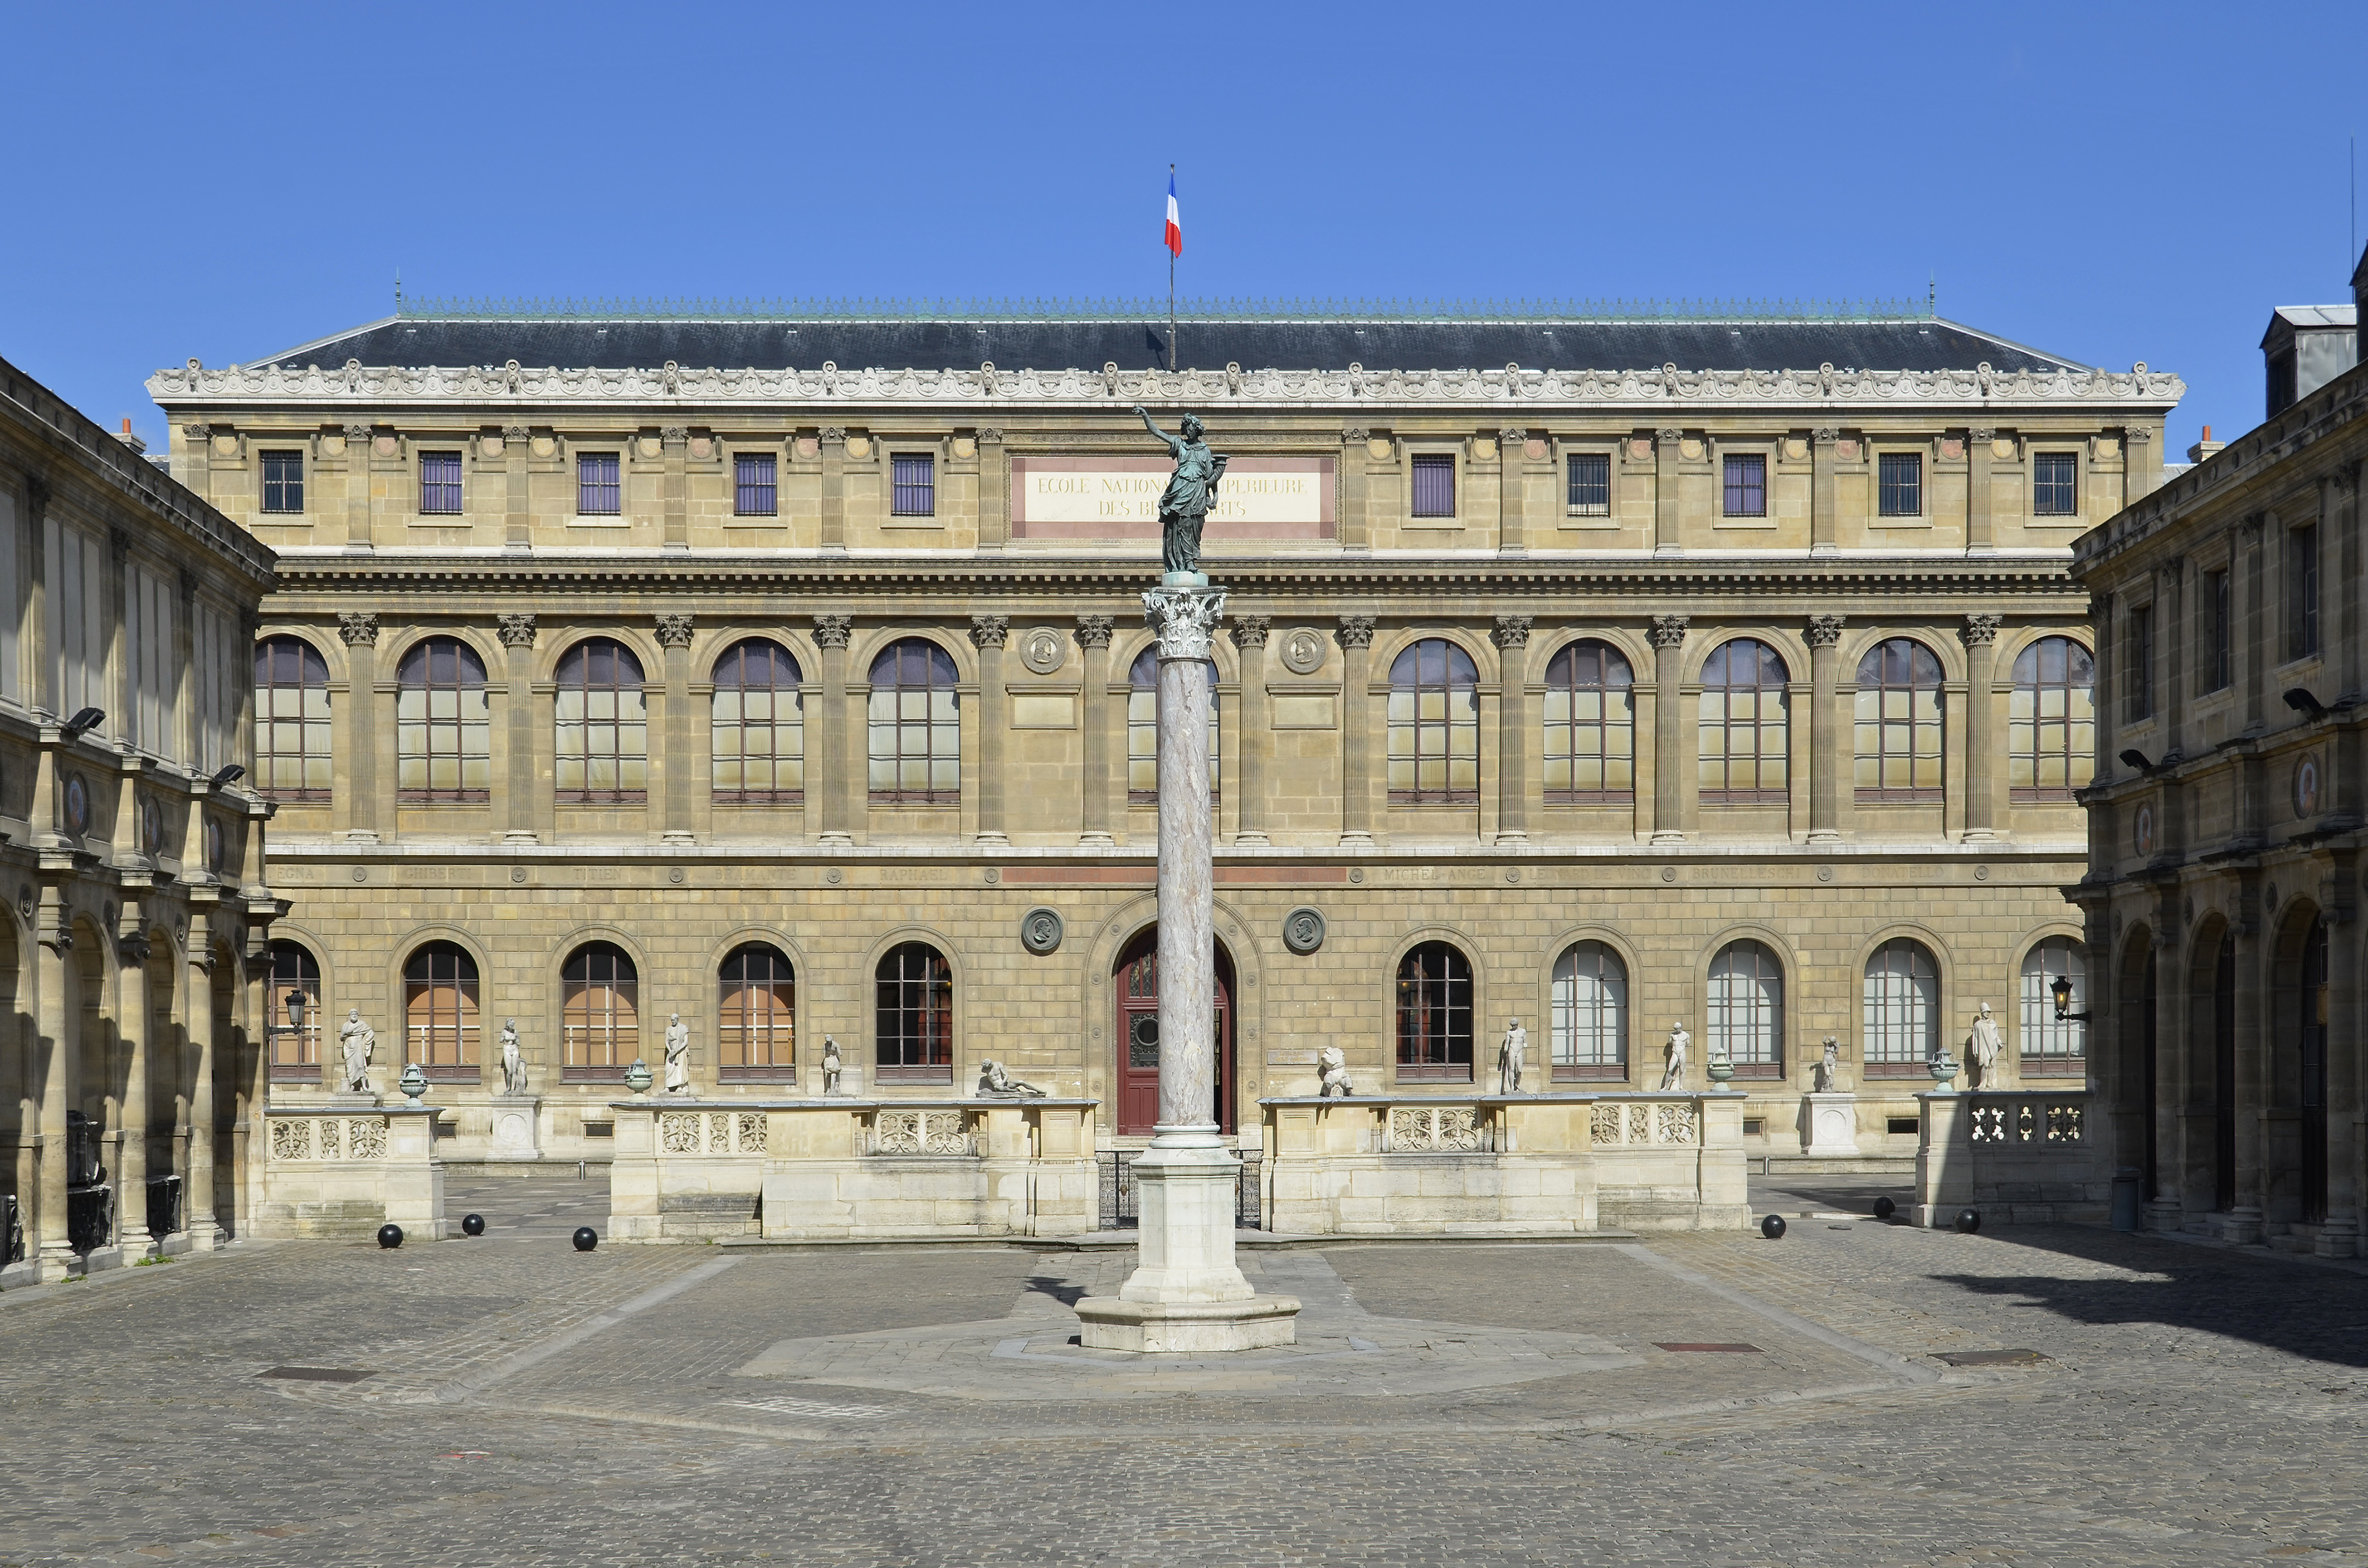
\includegraphics[height=1.2in]{img/chapter_6/beaux.jpg}
                                        \caption{ Beaux Arts Hall Building}
                                        \label{fig: Beaux Arts Hall Building}
                                \end{subfigure}
                                \begin{subfigure}{.4\textwidth}
                                        \centering
                                        \includegraphics[height=1.2in]{img/chapter_6/Beaux-Arts-floorplan.png}
                                        \caption{Beaux Arts Hall floor plan}
                                        \label{fig: Beaux Arts Hall floor plan}
                                \end{subfigure}
                                \caption{Beaux Arts Hall}
                                \label{fig: Beaux Arts Hall}
                        \end{figure}
                        \\
                        \noindent
                        Similarily, Villa Buildings from Mies Van der Rohe 
                        \begin{figure}[h]
                                \centering
                                \begin{subfigure}{.4\textwidth}
                                        \centering
                                        \includegraphics[height=1.5in]{img/chapter_6/Villa.jpg}
                                        \caption{Villa Building}
                                        \label{fig:Villa Building}
                                \end{subfigure}
                                \begin{subfigure}{.5\textwidth}
                                        \centering
                                        \includegraphics[height=1.5in]{img/chapter_6/Villa-floorplan.jpg}
                                        \caption{Villa floorplan}
                                        \label{fig:Villa floorplan}
                                \end{subfigure}
                                \caption{Villa Style Building and floor plan}
                                \label{fig:Villa Style Building and floor plan}
                        \end{figure}

                        \subsubsection{Technical Standpoint}
                                \begin{enumerate}[label=\alph*.]
                                        \item First of all, isolate all the walls of a given plan
                                        \item Calculate the thickness of the wall at each point 
                                        \item Output the histogram of wall thickness
                                        \item Also,compute variation of thickness to describe the wall texture
                                \end{enumerate}
                        \pagebreak
                        \begin{figure}[h]
                                \centering
                                \includegraphics[width=1\textwidth]{img/chapter_6/thickness_texture.png}
                                \caption{Thickness and Texture of the floorplan}
                                \label{fig: Thickness and Texture of the floorplan}
                        \end{figure}
                
                \subsection{Connectivity}
                        Connectivity is used to tackles room adjacency. It provides proximity of rooms to one another and it is a key dimension of a floor plan. Connection between the room through door and corridor defines the existence of connection between them. 

                        \subsubsection{Technical Standpoint}
                                \begin{enumerate}[label=\alph*.]
                                        \item Fenestration is arrangement, partitioning, designing of windows and doors in a buildings. By using fenestration, we can deduce the graph among rooms. 
                                        \item Connectivity metric is generated.
                                        \item Then, adjacency matrix is build.
                                        \item Finally, graph representation will be generated.
                                \end{enumerate}
                                This graph is used to compare floor plans taking into account the similarity of connection among rooms.
                        
                        \begin{figure}[h]
                                \centering
                                \includegraphics[width=1\textwidth]{img/chapter_6/connectivity.png}
                                \caption{Connectivity of room in floor plan}
                                \label{fig:Connectivity of room in floor plan}
                        \end{figure}
                \pagebreak
                \subsection{Circulation}
                        Circulation captures how people move across the floor plan. By extracting skeleton of circulation, we can both quantity and qualify people's movement across a floor plan. 

                        \subsubsection{Technical Standpoint}
                                \begin{enumerate}[label=\alph*.]
                                        \item Extract circulation of a given floor plan
                                        \item Sum its length along each direction for 0 to 360 degree
                                        \item The resulting histogram is used to compared against other floor plan's circulation.
                                \end{enumerate}
                       
                        \begin{figure}[h]
                                \centering
                                \includegraphics[width=.8\textwidth]{img/chapter_6/circulation.png}
                                \caption{Circulation of room in floor plan}
                                \label{fig:Circulation of room in floor plan}
                        \end{figure}
                \pagebreak
        \section{GAN used }
                For the given parcel, we have to generate the footprint, generate the room split and then furnishing the splited room. For each step, we plan to use the paired image translation i.e. pix2pix GAN.
                \subsection{pix2pix GAN (Paired Image Translation)}
                        Image to Image translation with Conditional Adversial Network is a general purpose solution to translate image to image. Here, image translation is paired image translation. It also learns a loss function to train this mapping. Here, it has auto loss formulation hence, it is general purpose. No need for hand-engineering the loss functions. \\
                        \begin{figure}[h]
                                \centering
                                \includegraphics[width=.5\textwidth]{img/chapter_6/GAN_example.png}
                                \caption{ Image to Image Translation using Conditional GAN}
                                \label{fig: Image to Image Translation using Conditional GAN}
                        \end{figure}
                        In conditional GANs, it learns mapping from observed image x along with the random noise vector z, and then produced the image z. 
                        \begin{equation}
                                G: \{x,y\} \rightarrow y
                        \end{equation}
                        Here, generator is trained to produced output that cannot be distinguished from real images by an adversially trained discriminator, also discriminator is trained to do as well as possible and detecting the generator's fakes images.\\
                        
                        \begin{figure}[h]
                                \centering
                                \includegraphics[width=.8\textwidth]{img/chapter_6/cGAN_model.png}
                                \caption{ GAN Model}
                                \label{fig: GAN Model}
                        \end{figure}

                        \subsubsection{Objective}
                                The objective function of conditional GAN can be expressed as:
                                \begin{equation}
                                        \mathcal{L}_{cGAN}\{G,D\} = \mathbb{E}_{x,y}[log D(x,y)] + \mathbb{E}_{x,z}[log(1-D(x,G(x,z)))]
                                \end{equation}
                                Here, G tries to minimize this objective against an adversial and D tries to maximize it.
                        \subsubsection{Network Architectures}
                                In Conditional GAN, both generator and discriminator use modules in the form of convolution-BatchNorm-ReLu. The Generator use the U-Net Architecture. U-Net Architecture is an encoder-decoder with skip connections between mirrored layers in the encoder and decoder stacks. \\
                                Generally, the skip connections is added between each layer i and n-i, where n is the total number of layers.
                                \begin{figure}[h]
                                        \centering
                                        \includegraphics[width=.8\textwidth]{img/chapter_6/Unet.png}
                                        \caption{Architecture of the generator}
                                        \label{fig:Architecture of the generator}
                                \end{figure}
        \section{Datasets and Color Code}
                For the training purpose using Conditional GAN, we need paired data set for conversion from one set of image to another set of image. Data set required for the training purpose are:
                \begin{enumerate}[label=\alph*.]
                        \item Paired data set between parcel and corresponding footprint
                        \item Paired data set between footprint and corresponding room split
                        \item Paired data set between room split and corresponding furnished data 
                        \item Furnished Data to wall segmentation data for segmentation of wall that will be used to generate the 3D models
                \end{enumerate}
                But, unfortunately we have only these dataset: 
                \begin{enumerate}[label=\alph*.]
                        \item ROBIN dataset\cite{chattopadhyay_2021} (Repository Of BuildIng plaNs)
                        \item CVC-FP\cite{de2015cvc} for parsing the floor plan that can be used for image segmentation
                \end{enumerate}
                \break
                \begin{figure}[h]
                        \centering
                        \begin{subfigure}{.33\textwidth}
                                \centering
                                \includegraphics[height=1.5in]{img/chapter_6/3room.jpg}
                                \caption{Three Room Floor Plan}
                                \label{fig:Three Room Floor Plan}
                        \end{subfigure}
                        \begin{subfigure}{.33\textwidth}
                                \centering
                                \includegraphics[height=1.5in]{img/chapter_6/4room.jpg}
                                \caption{Four Room Floor Plan}
                                \label{fig:Four Room Floor Plan}
                        \end{subfigure}
                        \begin{subfigure}{.3\textwidth}
                                \centering
                                \includegraphics[height=1.5in]{img/chapter_6/5room.jpg}
                                \caption{Five Room Floor Plan}
                                \label{fig:Five Room Floor Plan}
                        \end{subfigure}
                        \caption{Data set from ROBIN Dataset}
                        \label{fig:Data set from ROBIN Dataset}
                \end{figure}
                \begin{figure}[h]
                        \centering
                        \begin{subfigure}{.5\textwidth}
                                \centering
                                \includegraphics[height=1.5in]{img/chapter_6/2.png}
                                \caption{Floor Plan}
                                \label{fig:Floor Plan}
                        \end{subfigure}
                        \begin{subfigure}{.4\textwidth}
                                \centering
                                \includegraphics[height=1.5in]{img/chapter_6/2_gt_16.jpg}
                                \caption{Wall Segmented Image}
                                \label{fig:Wall Segmented Image}
                        \end{subfigure}
                        \caption{CVC-FP data set}
                        \label{fig:CVC-FP data set}
                \end{figure}
                Now, we have to prepare dataset that will be suitable for our purpose. And, the following task have to be done to prepare the dataset. 
                \begin{enumerate}[label=\alph*.]
                        \item Identify the furniture in the ROBIN datasets
                        \item Identify the room in the ROBIN datasets
                        \item Color code for the furniture in each room
                        \item Color code for the room in the building
                        \item Script that is used to convert the furnished data into color code of furniture
                        \item Script that is used to convert the furnished data into room color code
                        \item Script that is used generate foot print from the robin data
                        \item Using the foot print and the criterion of the footprint, parcel will be created
                \end{enumerate}
                \pagebreak
                \subsection{Types of Room}
                        There are total 5 types of room as mentioned in the ROBIN dataset. 
                        \begin{enumerate}[label=\alph*.]
                                \item Bedroom
                                \item Bathroom
                                \item Entry
                                \item Kitchen
                                \item Hall
                        \end{enumerate}
                \subsection{Types of Furniture}
                        There are all together 12 types of furniture as mention in the ROBIN dataset. They are illustrated in the figure \ref{fig:Types of Furniture and corresponding symbol}.
                        \begin{figure}[h]
                                \centering
                                \includegraphics[width=.8\textwidth]{img/chapter_6/furniture_in_ROBIN.png}
                                \caption{Types of Furniture and corresponding symbol}
                                \label{fig:Types of Furniture and corresponding symbol}
                        \end{figure}                
                \subsection{Color Coding}
                        Now, we have the furnished floor plan, all types of furniture and types of room. Now, we can prepare dataset. We are planning to prepare data set by using the python script which needs to be prepared. This script is supposed to help us in automation of preparation of the dataset. Before, preparing the dataset, we have to color code different furniture and room using the distinct and highly contrast color. For this, we plan to use Kelly's 22 colors of maximum contrast that can be used in color coding without risk of confusion. This helps our model to train without confusion.\\
                        The order of colours in Kelly’s list was planned so that there would be maximum contrast between colours in a set if the required number of colours were always selected in order from the top.
                        \pagebreak
                        \begin{figure}[h]
                                \centering
                                \includegraphics[width=1\textwidth]{img/chapter_6/kellycolor.png}
                                \caption{Kelly's 22 Color of Maximum Contrast}
                                \label{fig:Kelly's 22 Color of Maximum Contrast}
                        \end{figure}